\chapter{Teknik \textit{Divide and Conguer}}\label{ch:modul4}


\section{Pengenalan \textit{Divide and Conguer}}
\textit{Divide and Conguer} merupakan salah satu pendekatan dalam menyelesaikan permasalahan algoritma. \textit{Divide and Conguer} terdiri atas tiga langkah:
\begin{enumerate}
	\item \textbf{\textit{Divide}/Memisahkan} --- Memisahkan permasalahan yang ada menjadi permasalahan yang lebih kecil (\textit{subproblem}).
	\item \textbf{\textit{Conguer}/Menyelesaikan} --- Menyelesaikan setiap \textit{subproblem} yang ada secara rekursif. Jika \textit{subproblem} tersebut sangat kecil atau tak bisa dipisahkan lagi, maka diselesaikan secara langsung dengan menggunakan algoritma yang sederhana.
	\item \textbf{\textit{Combine}/Menggabungkan} --- Menggabungkan setiap solusi dari \textit{subproblem} yang telah diselesaikan menjadi sebuah solusi yang lengkap dan optimal.
\end{enumerate}




\section{\textit{Merge Sort}}
Algoritma \textit{Merge Sort} merupakan algoritma pengurutan yang mengikuti pendekatan \textit{Divide and Conguer}. Algoritma tersebut menggunakan 3 langkah dari \textit{Divide and Conguer} sebagai berikut:
\begin{enumerate}
	\item \textbf{\textit{Divide}} --- Membagi $n$ elemen/bilangan menjadi dua bagian dimana masing-masing adalah $n/2$. Setiap $n$ bilangan akan terus dibagi dua sampai habis atau bilangan tinggal 1 saja.
	\item \textbf{\textit{Conguer}} --- Mengurut setiap bagian secara rekursif menggunakan \textit{merge sort}. 
	\item \textbf{\textit{Combine}} --- Menggabungkan dua bagian yang telah diurut untuk menghasilkan satu bagian keseluruhan yang sudah terurut.
\end{enumerate}

Gambar \ref{fig:mergeSortIllustration} menggambarkan cara kerja Merge Sort terhadap 7 buah bilangan yang tak terurut. Di illustrasi tersebut \textit{array} yang memiliki 7 bilangan tak terurut dipecah-pecah sampai menjadi 1 buah bilangan atau panjang \textit{array} 1 ($A.length = 1$). Karena satu buah bilangan sudah merupakan bilangan yang terurut maka pecahan bilangan tersebut digabungkan sampai menjadi satu \textit{array} bilangan yang terurut. 

\begin{figure}[htbp]
	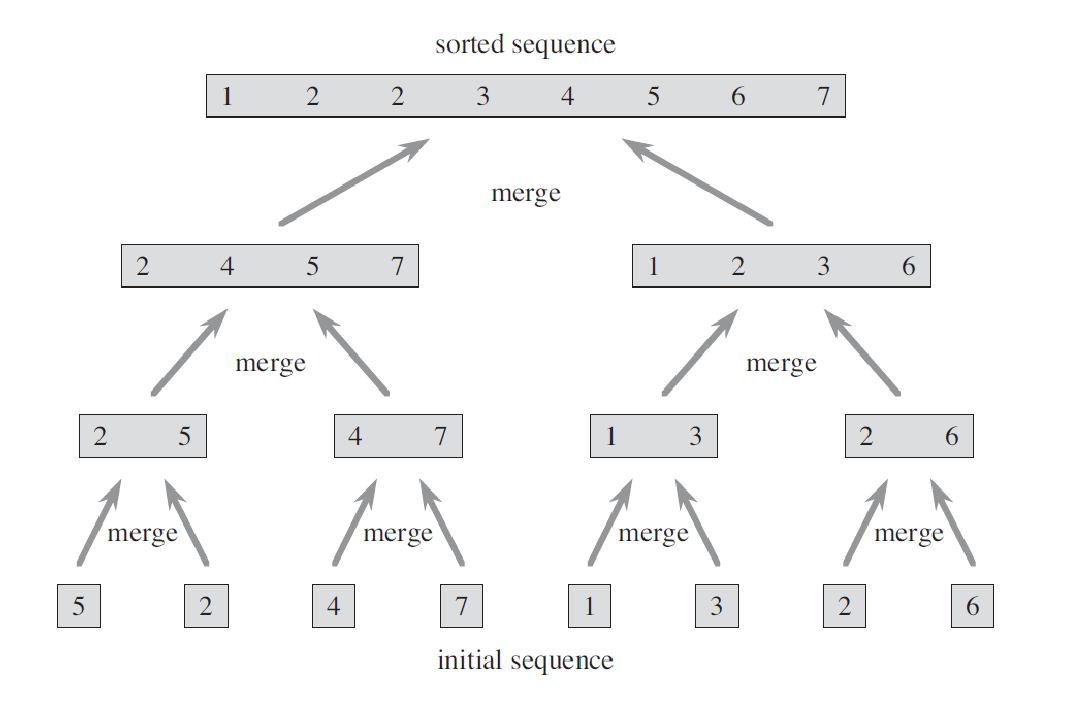
\includegraphics[scale=0.8]{fig/mergeSort1.eps}%
	\caption{Illustrasi dari cara kerja merge sort}%
	\label{fig:mergeSortIllustration}%
\end{figure}

Algoritma \textit{merge sort} terdiri dari dua algoritma utama yaitu Algoritma \ref{algo:merge} (MERGE($A,p,q,r$)) dan Algoritma \ref{algo:mergeSort} (MERGE-SORT($A,p,r$)). 

Algoritma MERGE-SORT($A,p,r$) ditujukan untuk membagi (\textit{divide}) sebuah \textit{array} $A$ menjadi dua bagian secara rekursif sampai \textit{array} tersebut tak bisa dibagi lagi (panjang \textit{array} $A$ adalah 1). 

Algoritma MERGE($A,p,q,r$) ditujukan untuk menggabungkan (\textit{combine}) kumpulan \textit{array} yang sudah diurut (memiliki panjang 1) menjadi sebuah \textit{array} baru yang sudah terurut.

Perlu diketahui di algoritma \textit{merge sort} tidak diperlukan fungsi khusus untuk \textit{conguer} dikarenakan \textit{array} yang memiliki panjang 1 secara otomatis sudah terurut.

\FloatBarrier
\begin{algorithm}[htbp]
	\caption{MERGE($A,p,q,r$)}
	\label{algo:merge}
	\begin{algorithmic}[1]
		\STATE $n_1 = q - p + 1$
		\STATE $n_2 = r - q$
		\STATE bentuk \textit{array} baru $L[1..n_1+1]$ dan $R[1..n_2+1]$.
		\FOR{$i = 1$ \TO $n_1$}
			\STATE $L[i] = A[p+i-1]$
		\ENDFOR
		\FOR{$j=1$ \TO $n_2$}
			\STATE $R[j] = A[q+j]$
		\ENDFOR
		\STATE $L[n_1+1] = \infty$
		\STATE $R[n_2+1] = \infty$
		\STATE $i=1$
		\STATE $j=1$
		\FOR{$k=p$ \TO $r$}
			\IF{$L[i]\leq{}R[j]$}
				\STATE $A[k] = L[i]$
				\STATE $i = i +1$
			\ELSE
				\STATE $A[k]=R[j]$
				\STATE $j=j+1$
			\ENDIF
		\ENDFOR
	\end{algorithmic}
\end{algorithm}

\begin{algorithm}[htbp]
	\caption{MERGE-SORT($A,p,r$)}
	\label{algo:mergeSort}
	\begin{algorithmic}[1]
		\IF{$p<r$}
			\STATE $q = \left\lfloor{}(p+r)/2\right\rfloor$
			\STATE MERGE-SORT($A,p,q$)
			\STATE MERGE-SORT($A,q+1,r$)
			\STATE MERGE($A,p,q,r$) 
		\ENDIF
	\end{algorithmic}
\end{algorithm}

\FloatBarrier
\begin{listprog}{mergeSort.py}
	\label{lst:mergeSort}
	\begin{lstlisting}[language=Python]
	def merge(A,p,q,r):
			n1 = q-p+1
			n2 = r-q
			L = []
			R = []
			for i in range(1,n1+1):
					L.append(A[p+i-1])
			for j in range(1,n2+1):
					R.append(A[q+j])
			L.append(float('inf'))
			R.append(float('inf'))
			i = 0
			j = 0
			for k in range(p,r+1):
					if L[i]<=R[j]:
							A[k] = L[i]
							i += 1
					else:
							A[k] = R[j]
							j += 1

	def mergeSort(A,p,r):
			if p<r:
					q = int((p+r)/2)
					mergeSort(A,p,q)
					mergeSort(A,q+1,r)
					merge(A,p,q,r)

	A = [1,4,7,2,3]
	mergeSort(A,0,4)
	print A
	\end{lstlisting}
\end{listprog}

\FloatBarrier

\section{Permasalahan Pencarian Minimum dan Maksimum}
Diberikan sebuah rangkaian bilangan, bagaimana cara paling cepat untuk mencari bilangan terbesar dan terkecil dari rangkaian tersebut? 

Untuk menyelesaikan masalah tersebut, ada beberapa pendekatan. Pendekatan yang naif adalah dengan melakukan \textit{looping} dari awal rangkaian sampai akhir rangkaian yang diperlihatkan di Algoritma \ref{algo:minmaxnaif}. Sedangkan untuk pendekatan \textit{Divide and Conguer} bisa dilihat di Algoritma \ref{algo:minmaxdac}.

\begin{algorithm}[H]
	\caption{MIN-MAX-NAIF($A$)}
	\label{algo:minmaxnaif}
	\begin{algorithmic}[1]
		\STATE $min = A[1]$
		\STATE $max = A[1]$
		\FOR{$i=2$ \TO $A.length$}
			\IF{$A[i] < min$}
				\STATE $min = A[i]$
			\ENDIF
			\IF{$A[i] > max$}
				\STATE $max = A[i]$
			\ENDIF
		\ENDFOR
		\RETURN $min,max$
	\end{algorithmic}
\end{algorithm}

Algoritma \ref{algo:minmaxnaif} memiliki jumlah komparasi sebanyak $2n-2$. Akan tetapi dengan menggunakan strategi \textit{divide and conquer} jumlah komparasi yang dilakukan bisa dikecilkan menjadi $(3n/2)-2$. Ini mungkin tidak signifikan, walaupun demikian untuk kasus lain strategi \textit{divide and conguer} bisa mengurangi jumlah instruksi secara drastis. 

Algoritma \ref{algo:minmaxdac} menggunakan strategi \textit{divide and conquer} untuk mencari nilai minimum dan maksimum dari rangkaian angka. Prinsipnya adalah dengan membagi rangkaian angka tersebut menjadi dua bagian yaitu $A[1..n/2]$ dan $A[(n/2)+2..n]$, mencari minimum dan maksimum di kedua bagian tersebut, dan terakhir mengambil minimum terkecil dari maksimum terbesar dari kedua bagian tersebut.

\begin{algorithm}[H]
	\caption{MIN-MAX-DAC($A$,$low$,$high$)}
	\label{algo:minmaxdac}
	\begin{algorithmic}[1]
		\IF{$high - low = 1$}
			\IF{$A[low] < A[high]$}
				\RETURN ($A[low]$,$A[high]$)
			\ELSE
				\RETURN ($A[high]$,$A[low]$)
			\ENDIF
		\ELSE
			\STATE $mid = \left\lfloor (low+high)/2\right\rfloor$
			\STATE $x_1,y_1$ = MIN-MAX-DAC($A$,$low$,$mid$)
			\STATE $x_2,y_2$ = MIN-MAX-DAC($A$,$mid+1$,$high$)
			\IF{$x_1 < x_2$}
				\STATE $x = x_1$
			\ELSE
				\STATE $x = x_2$
			\ENDIF
			\IF{$y_1 < y_2$}
				\STATE $y = y_1$
			\ELSE
				\STATE $y = y_2$
			\ENDIF  
			\RETURN $(x,y)$
		\ENDIF
	\end{algorithmic}
\end{algorithm}



\section{\textit{Binary Search}}

\textit{Binary Search} merupakan metode pencarian elemen di suatu rangkaian tertentu dengan menggunakan strategi \textit{divide and conquer}. Worst case \textit{binary search} adalah $O(log n)$ dimana jumlah komparasi terbanyak yang dilakukan adalah sebanyak $\left\lfloor log n \right\rfloor + 1$ untuk $n$ input.

\begin{algorithm}[H]
	\caption{BINARY-SEARCH($A,low,high,x$)}
	\begin{algorithmic}[1]
		\IF{$low > high$}
			\RETURN 0
		\ELSE
			\STATE $mid = \left\lfloor(low+high)/2)\right\rfloor$
			\IF{$x==A[mid]$}
				\RETURN $mid$
			\ELSIF{$x<A[mid]$}
				\RETURN BINARY-SEARCH($A,low,mid-1,x$) 
			\ELSE
				\RETURN BINARY-SEARCH($A,mid+1,high,x$)
			\ENDIF
		\ENDIF
	\end{algorithmic}
\end{algorithm}



\section{\textit{Quick Sort}}

\textit{Quick sort} seperti \textit{merge sort} juga menggunakan pendekatan \textit{Divide and Conguer}. Tiga langkah yang dimiliki \textit{quick sort} ialah:
\begin{enumerate}
	\item \textit{Divide} --- Mempartisi (menyusun) \textit{array} $A[p..r]$ menjadi dua \textit{subarray} yang berukuran lebih kecil yaitu $A[p..q-1]$ dan $A[q+1..r]$ sehingga setiap elemen dari $A[p..q-1]$ lebih kecil atau sama dengan $A[q]$ yang mana akan lebih kecil atau sama dari setiap elemen $A[q+1..r]$. Indeks $q$ dihitung melalui fungsi partisi.
	\item \textit{Conguer} --- Urut dua \textit{subarray} $A[p..q-1]$ dan $A[q+1..r]$ secara rekursif.
	\item \textit{Combine} --- Tahap ini tidak perlu dilakukan karena sudah tergabung secara otomatis.
\end{enumerate}

\begin{algorithm}[H]
	\caption{QUICKSORT($A,p,r$)}
	\begin{algorithmic}[1]
		\IF{$p<r$}
			\STATE $q$ = PARTITION($A,p,r$)
			\STATE QUICKSORT($A,p,q-1$)
			\STATE QUICKSORT($A,q+1,r$)
		\ENDIF
	\end{algorithmic}
\end{algorithm}

\begin{algorithm}[H]
	\caption{PARTITION($A,p,r$)}
	\begin{algorithmic}[1]
		\STATE $x = A[r]$
		\STATE $i = p-1$
		\FOR{$j=p$ \TO $r-1$}
			\IF{$A[j] <= x$}
				\STATE $i = i + 1$
				\STATE $temp = A[i]$
				\STATE $A[i] = A[j]$
				\STATE $A[j] = temp$
			\ENDIF
		\ENDFOR
		\STATE $temp = A[i+1]$
		\STATE $A[i+1] = A[r]$
		\STATE $A[r] = temp$
		\RETURN $i+1$
	\end{algorithmic}
\end{algorithm}

Sebuah variasi dari algoritma \textit{quick sort} adalah algoritma \textit{randomized-quick sort} dimana di algoritma tersebut pemilihan variabel \textit{q} dilakukan secara acak (\textit{random}). Hal tersebut dilakukan dengan harapan pemotongan rangkaian (\textit{partition}) lebih terdistribusi secara merata.

\begin{algorithm}[H]
	\caption{RANDOMIZED-PARTITION($A,p,r$)}
	\begin{algorithmic}[1]
		\STATE $i$ = RANDOM($p$,$r$)
		\STATE exchange $A[r]$ with $A[i]$
		\RETURN PARTITION($A,p,r$)
	\end{algorithmic}
\end{algorithm}

\begin{algorithm}[H]
	\caption{RANDOMIZED-QUICKSORT($A,p,r$)}
	\begin{algorithmic}[1]
		\IF{$p<r$}
			\STATE $q$ = RANDOMIZED-PARTITION($A,p,r$)
			\STATE RANDOMIZED-QUICKSORT($A,p,q-1$)
			\STATE RANDOMIZED-QUICKSORT($A,q+1,r$)
		\ENDIF
	\end{algorithmic}
\end{algorithm}